

\documentclass[english,11pt]{beamer}

\DeclareMathOperator{\Cov}{Cov}
\DeclareMathOperator{\Var}{Var}
\DeclareMathOperator{\E}{\mathbb{E}}
\DeclareMathOperator{\Proba}{\mathbb{P}}

\newcommand{\Covb}[2]{\ensuremath{\Cov\!\left[#1,#2\right]}}
\newcommand{\Eb}[1]{\ensuremath{\E\!\left[#1\right]}}
\newcommand{\Pb}[1]{\ensuremath{\Proba\!\left[#1\right]}}
\newcommand{\Varb}[1]{\ensuremath{\Var\!\left[#1\right]}}

% norm
\newcommand{\norm}[1]{\| #1 \|}

\newcommand{\indep}{\rotatebox[origin=c]{90}{$\models$}}





\usepackage{mathptmx,amsmath,amssymb,graphicx,bibentry,bbm,babel,ragged2e}

\makeatletter

\newcommand{\noun}[1]{\textsc{#1}}
\newcommand{\jitem}[1]{\item \begin{justify} #1 \end{justify} \vfill{}}
\newcommand{\sframe}[2]{\frame{\frametitle{#1} #2}}

\newenvironment{centercolumns}{\begin{columns}[c]}{\end{columns}}
%\newenvironment{jitem}{\begin{justify}\begin{itemize}}{\end{itemize}\end{justify}}

\usetheme{Warsaw}
\setbeamertemplate{footline}[text line]{}
\setbeamertemplate{headline}{}
\setbeamercolor{structure}{fg=purple!50!blue, bg=purple!50!blue}

\setbeamersize{text margin left=15pt,text margin right=15pt}

\setbeamercovered{transparent}


\@ifundefined{showcaptionsetup}{}{%
 \PassOptionsToPackage{caption=false}{subfig}}
\usepackage{subfig}

\usepackage[utf8]{inputenc}
\usepackage[T1]{fontenc}

\usepackage{multirow}

\usepackage{mdframed}


%\AtBeginSection[]
%{
%  \begin{frame}
%  \frametitle{}
%  \tableofcontents[currentsection]
%  \end{frame}
%}

\makeatother




\begin{document}

\title
[A generative model for urban firm networks]{A generative model for urban firm networks}
\author[Raimbault \and Zdanowska \and Arcaute]{J.~Raimbault$^{1,2,3\ast}$ \and N. Zdanowska$^{1,3}$ \and E. Arcaute$^{1}$\\\medskip
$^{\ast}$\texttt{j.raimbault@ucl.ac.uk}
}

\institute[UCL]{$^{1}$CASA, UCL\\
$^{2}$UPS CNRS 3611 Complex Systems Institute Paris\\
$^{3}$UMR CNRS 8504 G{\'e}ographie-cit{\'e}s
}




\date[24 September 2020]{NetSci\\
September 24 2020
}

\frame{\maketitle}

\section{Introduction}


\sframe{Urban firm networks}{


General framework:

\begin{itemize}
\item Cities as cross-overs of socio-economic interactions           \cite{castells1996information}
    \item Networks as the new social morphology of societies \cite{castells2000networksociety}, giving rise to network economies \cite{sassen1991global} 
    \item Emergence of an interconnected world city network as a crucial feature of globalisation 
    \item Interurban interactions between firms as one of the most representative of economic trends \cite{taylor2001specification} \cite{martinus2018global}
    
\end{itemize}

\bigskip

}


\sframe{An evolutionary approach to Urban Systems}{

\begin{itemize}
    \item Evolutionary Theory of Urban Systems \cite{pumain1997pour} \cite{pumain2006villes}
    \item Adaptive cycles and diffusion of innovation \cite{Hagerstrand1968Innovation}
    \item Path dependence \cite{martin2006path} \cite{pumain2012urban}
    \item Selection and emerging structures of systems 
    \item Evolutionary models for urban systems dynamics: \cite{favaro2011gibrat} \cite{cottineau2015growing} \cite{schmitt2015half} \cite{raimbault2018indirect} \cite{raimbault2018calibration}
\end{itemize}

}

\sframe{Urban firm linkages and geo-economic processes}{

Assumptions

\begin{itemize}
    \item Metropolisation vs. regionalisation effects
    \item Relationship local/global of multinational firm linkages 
    \item Specialisation-driven factors and drivers of innovation
    \item Macroeconomic exogenous chocs and resilience of urban systems 
\end{itemize}

\bigskip

$\rightarrow$ \textit{How can we capture geographical and economic processes within urban networks of firms with a generative model?}

\begin{itemize}
	\item Indirect inference on processes
	\item Includes path-dependency
\end{itemize}


}

\section{Model}

\sframe{Model rationale}{

$\rightarrow$ Cities are defined by their GDP and their profile regarding the proportion of firms in the different sectors. Links between cities are created in an iterative way, taking into account:

\medskip

    \begin{itemize}
        \item geographical proximity (distance or effective accessibility)
        \item geopolitical proximity (belonging to the same country or single market $\rightarrow$ application to Brexit)
        \item city size (economic size as GDP) 
        \item economic similarity (e.g. cosine distance between sector proximity as done in \cite{2019arXiv190505106C}
        \item previous linkages 
    \end{itemize}

}


\sframe{Formalization}{

Cities characterized by economic size $E_i$ (GDP) and economic structure $S_{ik}$ (probability distribution of firms within $K$ sectors)

% Le k c'est bien le nombre de secteurs? 
% -> oui exactement


\bigskip

Starting from an initial network, at each time step:
\begin{enumerate}
    \item Evolve city sizes $E_i \left(t \textrm{ + } 1 \right) \textrm{ = } f\left(E_j\left(t\right)\right)$ with an interaction model (\cite{raimbault2018indirect} or \cite{cottineau2015growing})
    % ici le = n'apparait pas dans la formule. le t c'est bien le temps?
    %  => oui t est le temps ; les = et + et ( ) qui passent pas c'est la template ucl, j'arrive pas a fixer alors il faut passer par le reswitch en mode texte
    \item Add a fixed number of links randomly, following a probability function of sizes, sector proximity, and geographical and socio-cultural proximity
\end{enumerate}

}


\sframe{Formalization}{

Probability for a new link follows a generalized Cobb-Douglas function

\medskip

\[
     p_{ij} \propto \left(\frac{E_{i}}{E}\right)^{\gamma_F} \cdot \left(\frac{E_{j}}{E}\right)^{\gamma_T} \cdot \left(\frac{w_{ij}}{W}\right)^{\gamma_W} \cdot s\left(S_{ik},S_{jk}\right)^{\gamma_S} \cdot \exp \left(- \gamma_G \cdot d_{ij}\right) \cdot \exp \left(- \gamma_D \cdot g_{ij}\right)
\]



\medskip

where $E \textrm{ = } \sum_k E_k$, $W \textrm{ = } \sum_{i,j} w_{ij}$, $s$ is a proximity measure given by cosine similarity, $d_{ij}$ euclidian distance, and $g_{ij}$ a socio-cultural distance

\bigskip
\bigskip

\textbf{Model parameters: } $\gamma_F, \gamma_T, \gamma_W, \gamma_S, \gamma_D \textrm{ = } \frac{1}{d_G}, \gamma_G \textrm{ = } \frac{1}{d_G}$

}

\sframe{Model indicators}{

\textbf{Geographical indicators:}

\begin{itemize}
    \item Internationalisation (modularity of countries in the network)
    \item Metropolisation (correlation between weighted degree and city size)
    \item Regionalisation (correlation between length and flow of links, stratified by size of extremities)
    \item Specialisation (correlation between sector proximity and flow of links, stratified by size of extremities)
\end{itemize}

\bigskip

\textbf{Network and flows indicators:}

%  networkModularity, networkAvgCommunitySize, networkDegreeHierarchy, networkAvgDegree, networkDegreeEntropy, flowsHierarchy, flowsEntropy, rhoDegreeSize, rhoFlowDistancePos, rhoFlowDistance

\begin{itemize}
    \item Louvain modularity, community sizes
    \item Degree and flows distribution (average, hierarchy, entropy)
    \item Correlations (degree-size, flow-distance)
\end{itemize}

}

\sframe{Simulation on synthetic systems of cities}{


\justify
 
\textit{Following \cite{raimbault2018space}, geosimulation models must be studied within synthetic controllable urban contexts in order to (i) understand intrinsic behavior of the model and robust qualitative stylized facts; (ii) study the sensitivity to the spatial configuration}

\bigskip

Generation of a continent-scale urban system with stylized order of magnitude corresponding to Europe:

\medskip

\footnotesize

\begin{enumerate}
    \item Generate $N \textrm{ = } 700$ cities with size following a power law $E_i \textrm{ = } E_0 \cdot i^{-\alpha}$ with $E_0 \textrm{ = } 10^{11}$ and $\alpha \textrm{ = } 1.1$ (computed on Europe for GDP with cities larger than 50.000 inhabitants)
    \item Distribute them randomly in space (\cite{simini2019testing} vs \cite{banos2011christaller})
    \item Create countries with k-means clustering ($C \textrm{ = } 30$)
    \item Distribute sectors such that (i) smaller cities are more specialized and (ii) larger cities are more knowledge-based, with a one dimensional axis to position sectors $1/K \ldots 1$ where the density $f\left(k\right)$ follows a log-normal with $\left(\mu,\sigma\right)$ such that $\sqrt{\Var f} \textrm{ = } K/2$ for the largest, $\sqrt{\Var f} \textrm{ = } 1/K$ for the smallest
\end{enumerate}

 
}

\section{Results}

\sframe{Implementation and experiments}{

\textbf{Implementation}

\begin{itemize}
	\item Model implemented in NetLogo (good compromise interactivity / ergonomy), with fast data structures (matrix/table extensions)
	\item Integrated seamlessly into OpenMOLE \cite{reuillon2013openmole} for model exploration (NetLogoTask)
\end{itemize}


\medskip

\textbf{Experiments}

% for now no dynamics of cities

\begin{itemize}
	\item Current experiment: only network dynamics (short time scale)
	\item One-factor sampling with 100 repetitions to assess statistical properties (good convergence, average sharpe ratios for indicators all larger than 5)
	\item Grid sampling with 20 repetitions for model behavior %(2years 5months of computation)
\end{itemize}

}

\sframe{Simulation of urban networks} 

{
    % examples
    
    \begin{center}
    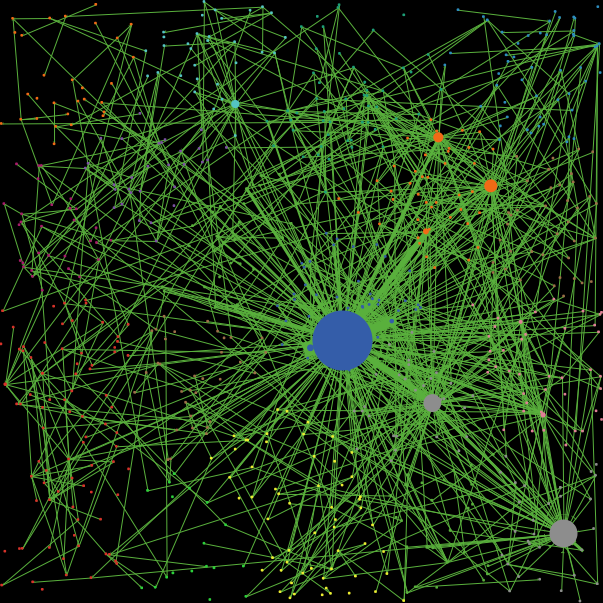
\includegraphics[width=0.48\textwidth]{figuresraw/ex_alleq-highgravity_seed-12102_t1500.png}\hspace{0.1cm}
    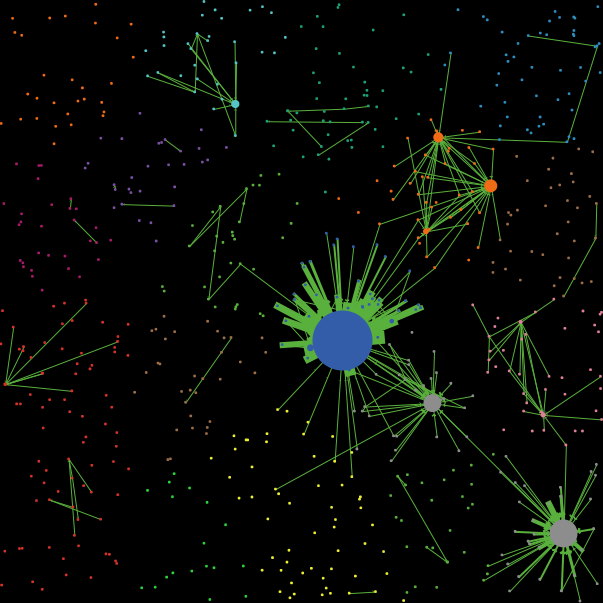
\includegraphics[width=0.48\textwidth]{figuresraw/ex_alleq-lowgravity_seed-12102_t1500.png}
	\end{center}

	\medskip

	\textit{Networks at $t \textrm{ = } 1500$, for default parameters values and high gravity (left) and low gravity (right)}

}

%\sframe{Statistical convergence}{

%$\rightarrow$ Good convergence for most indicators: average sharpes ratios on a one-factor sampling above 5 (except for metropolization index $\simeq 1.5$)

% + histograms

%\bigskip
%}


\sframe{Effect of interaction decay}{
    
    % One factor sampling results
    %  20190924_162740_ONEFACTOR_REPLICATIONS_SYNTHETIC_GRID
    
    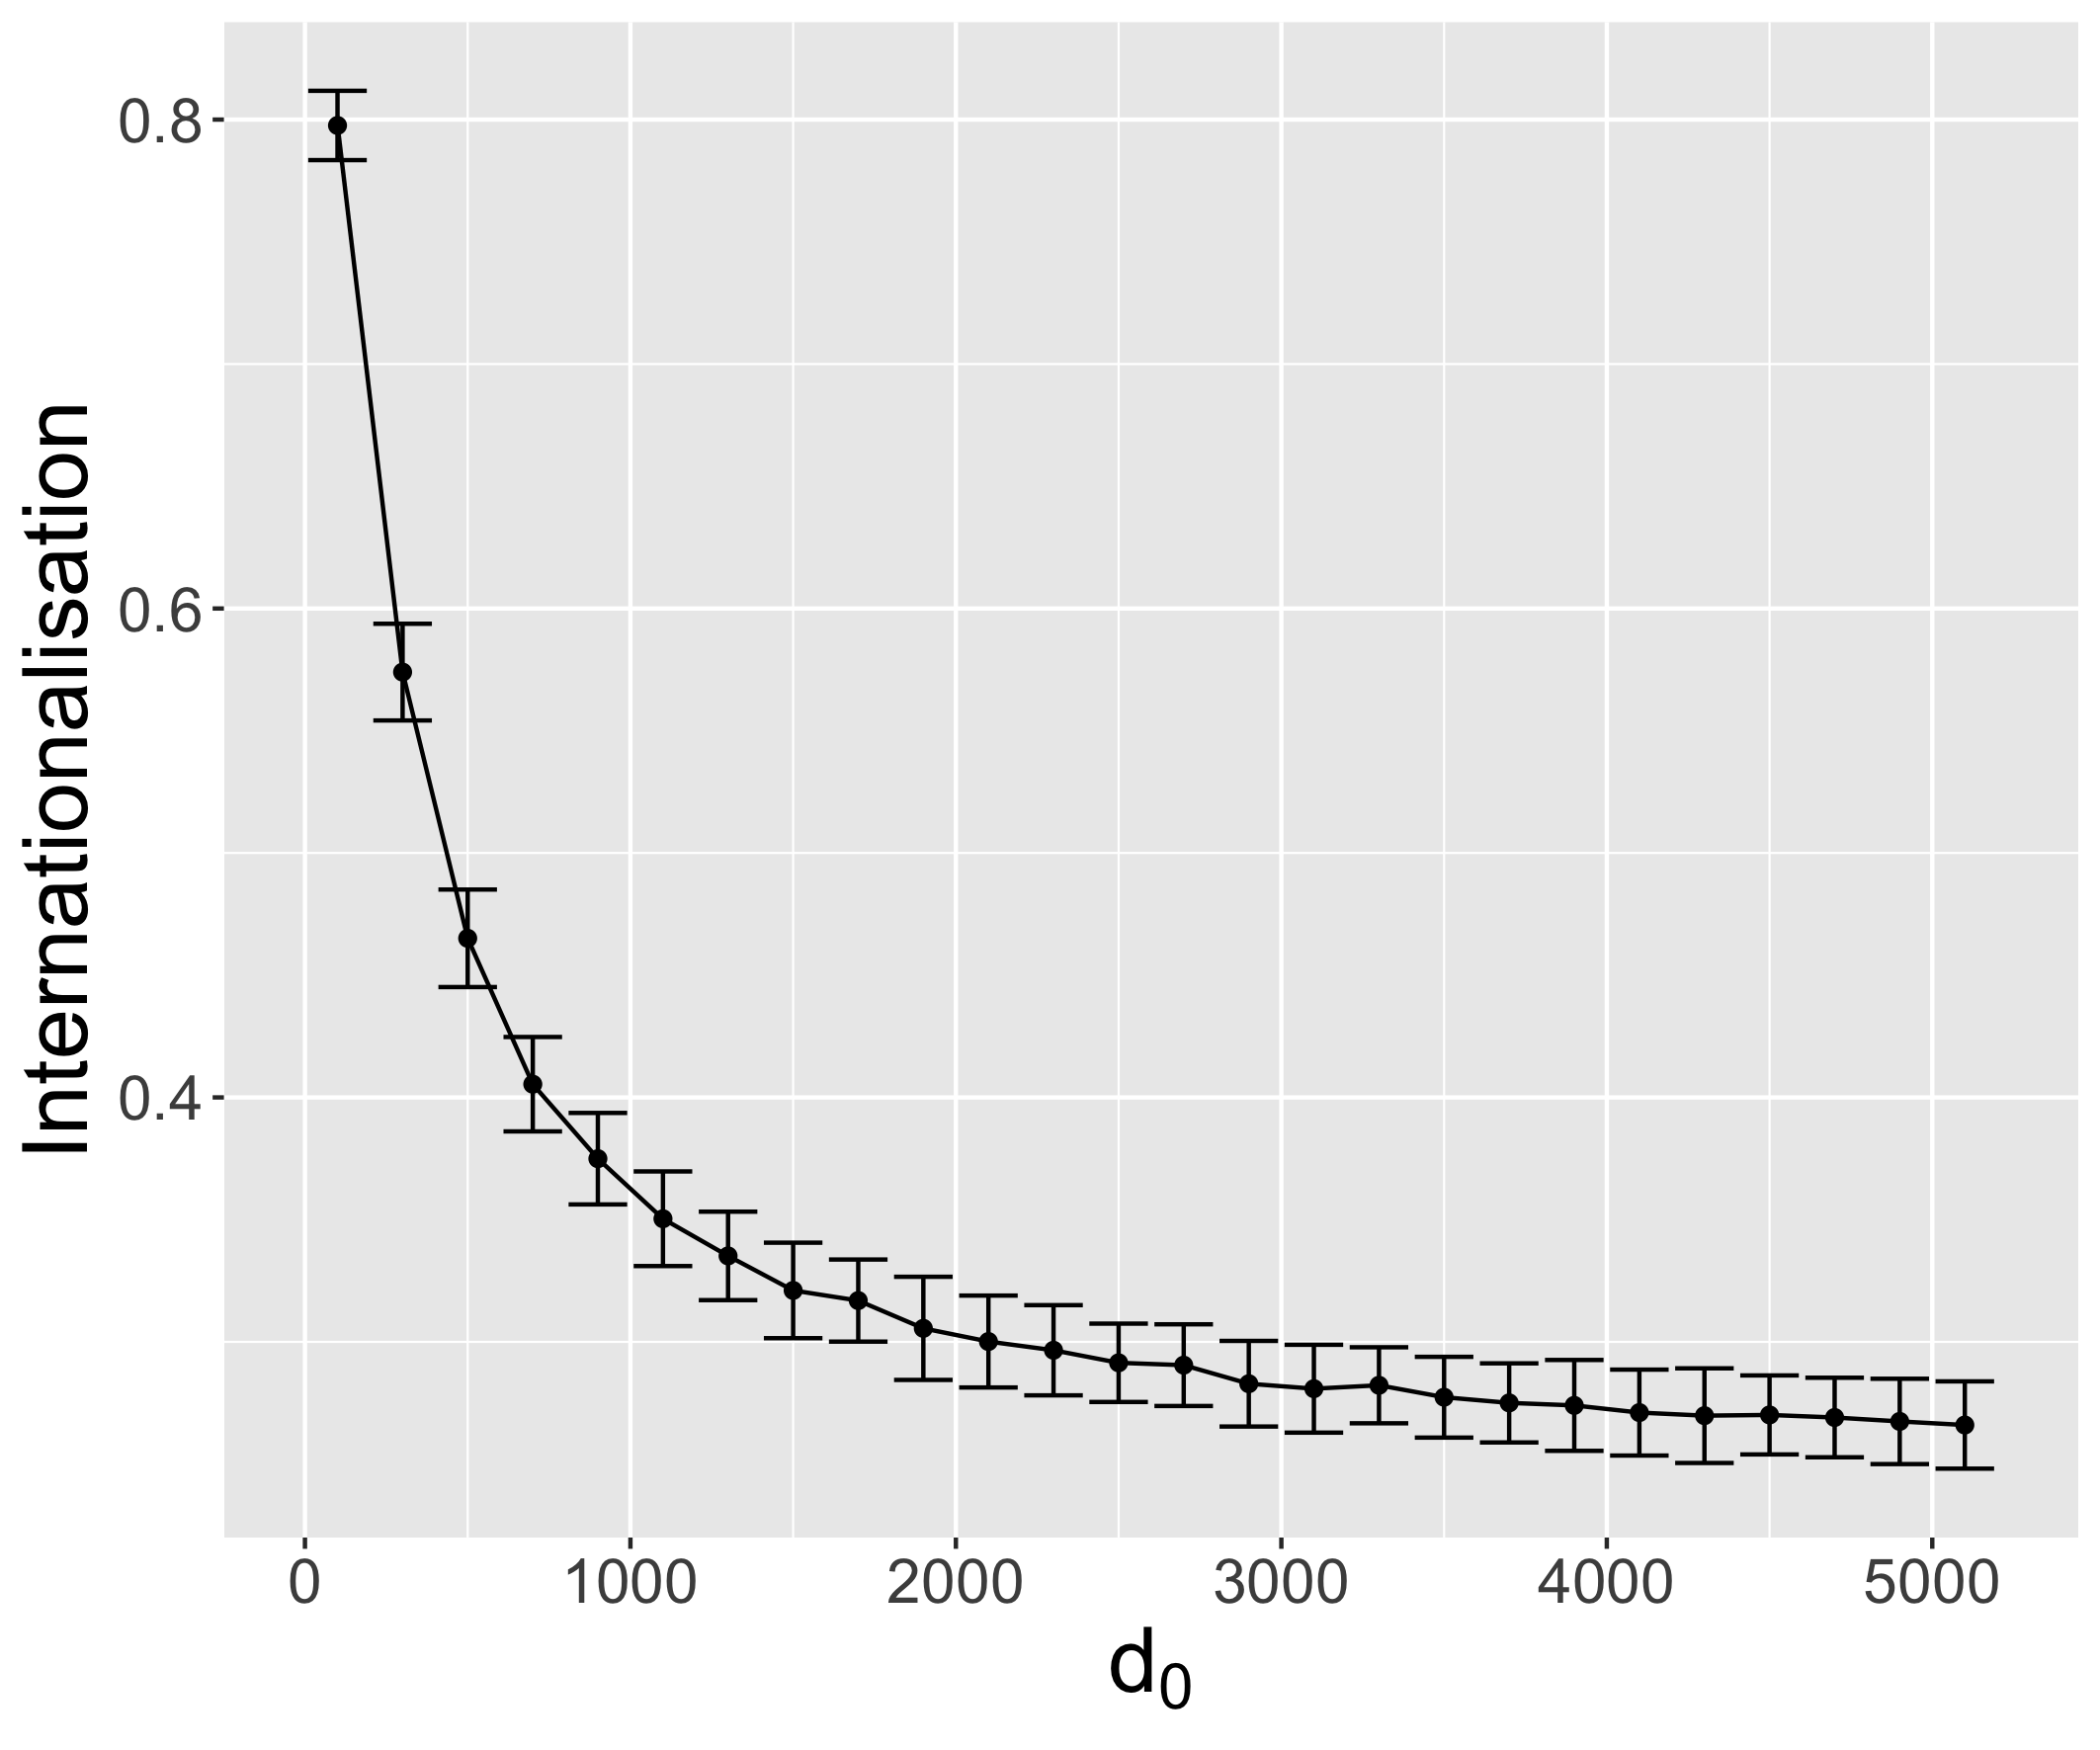
\includegraphics[width=0.48\textwidth]{figuresraw/internationalisation-gravityDecay_errorbars.png}
    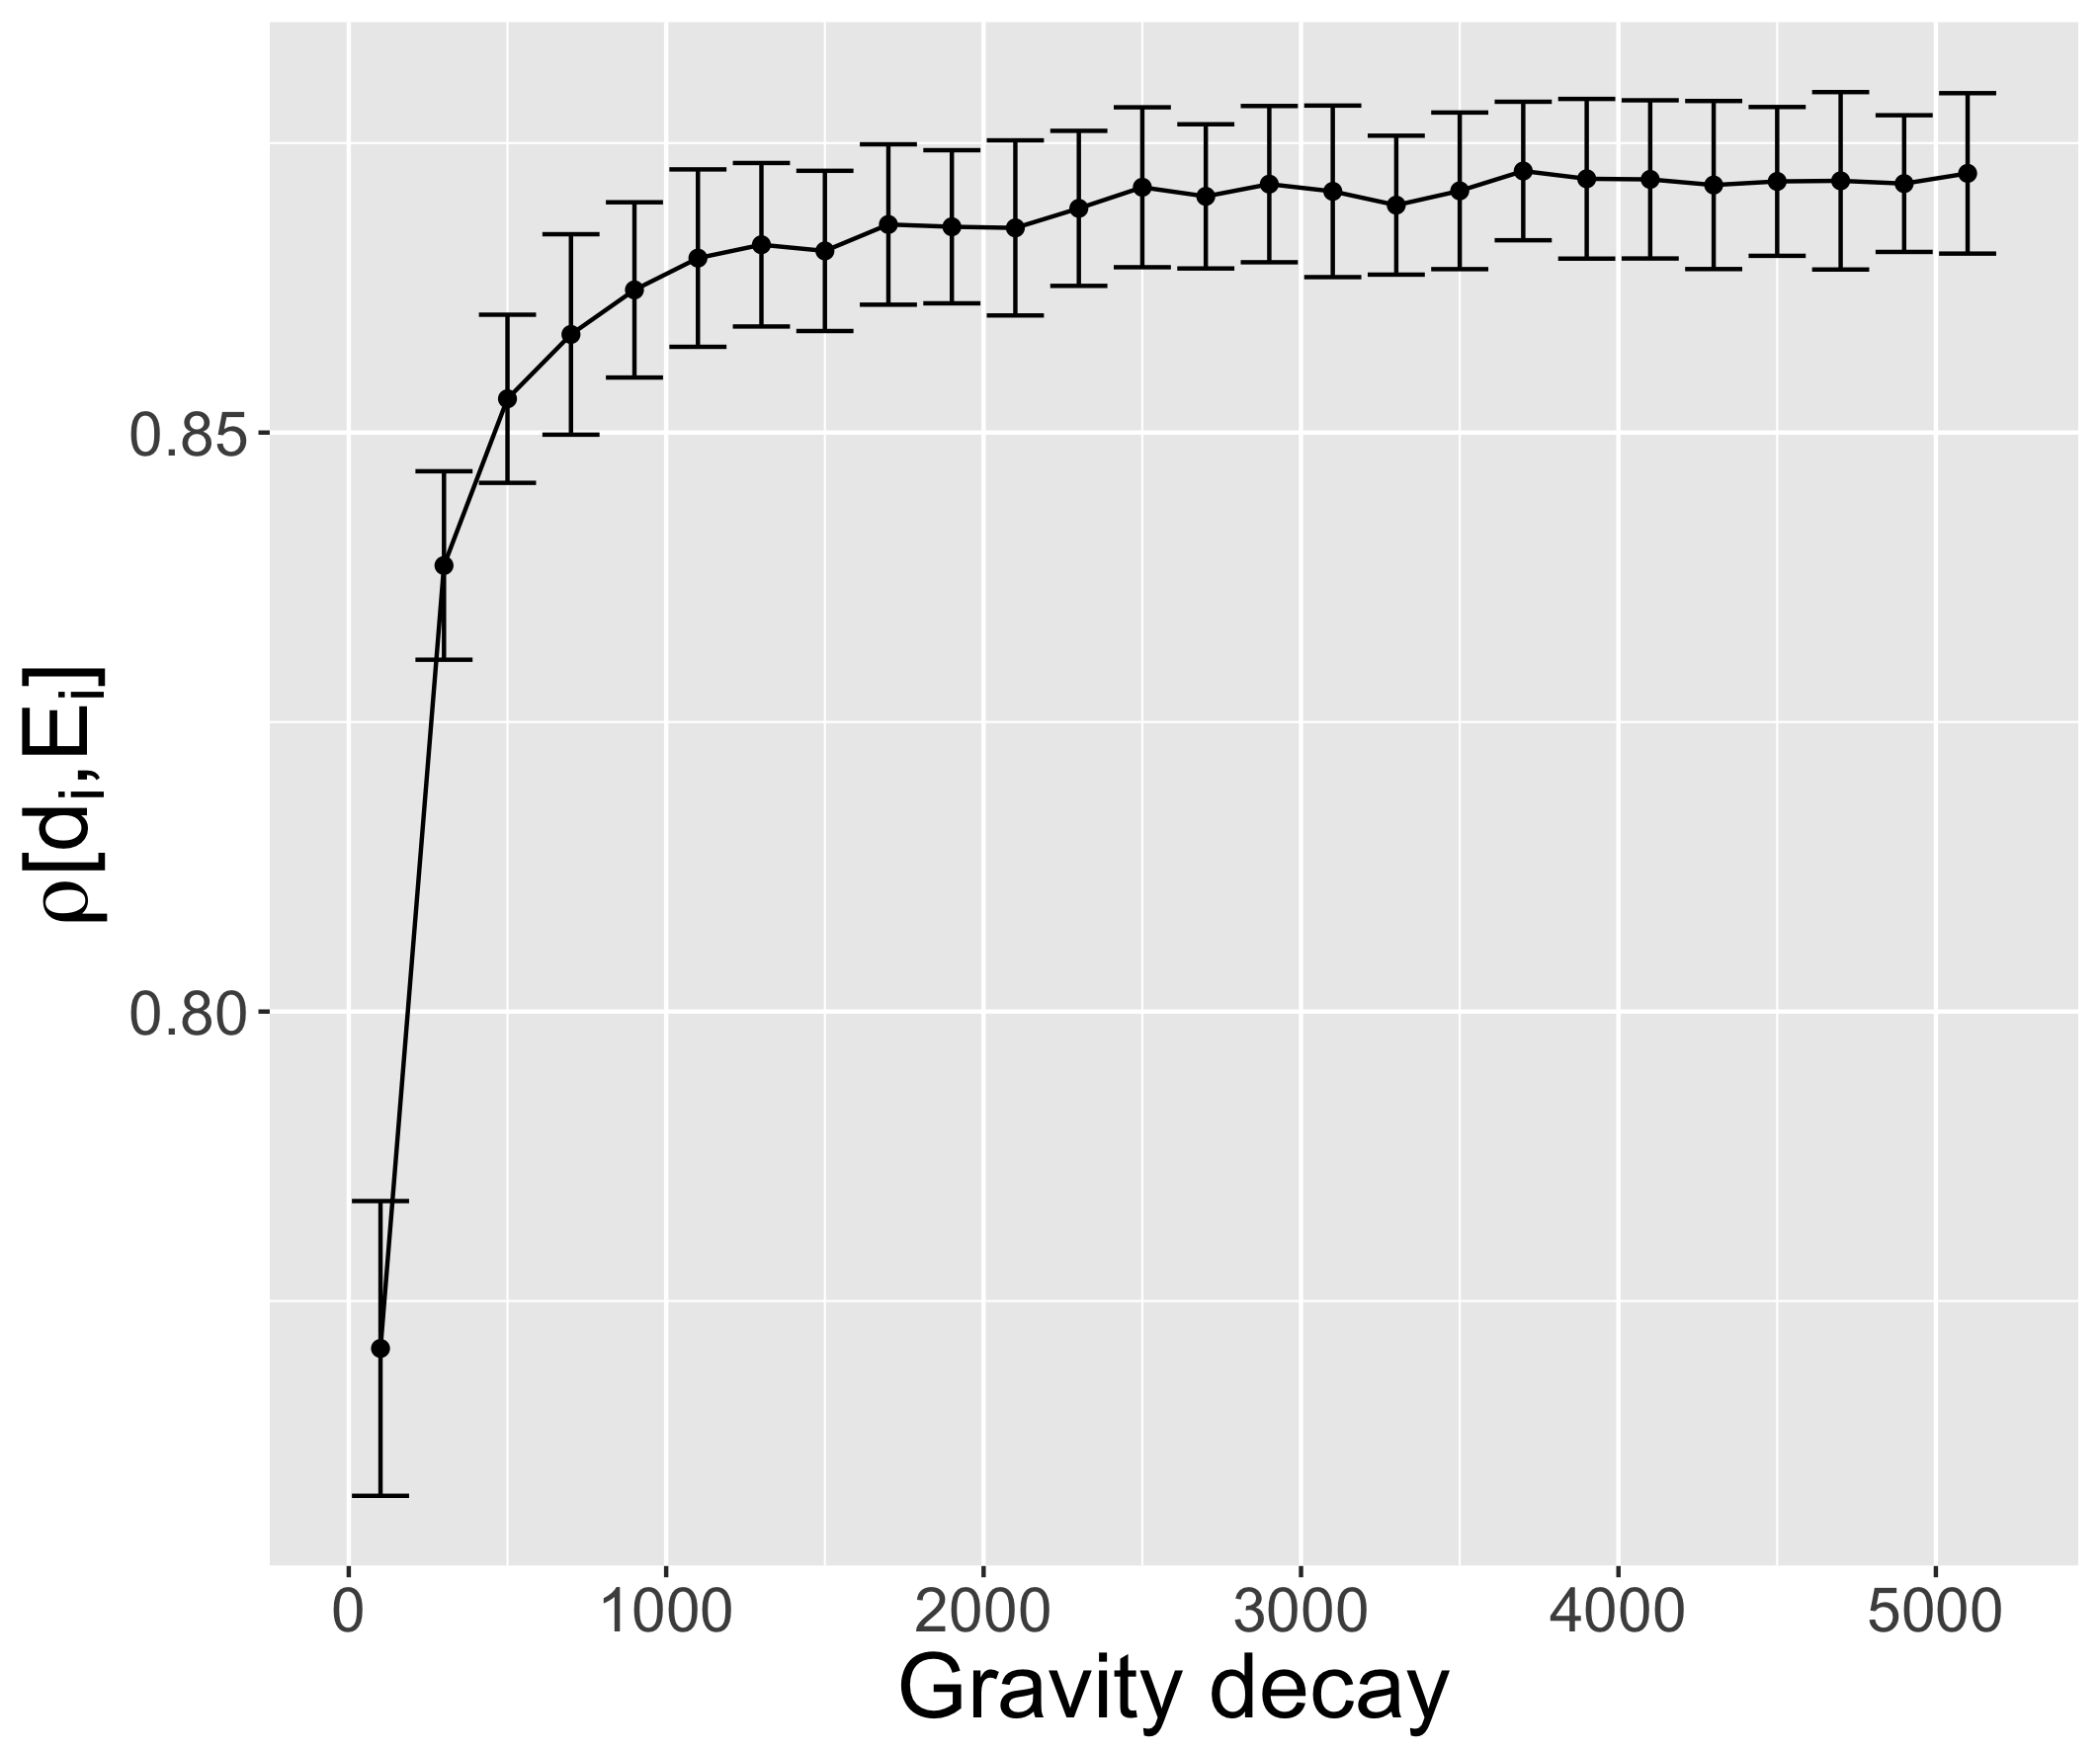
\includegraphics[width=0.48\textwidth]{figuresraw/rhoDegreeSize-gravityDecay_errorbars.png}
    
    \medskip
    
    \footnotesize
    
    \textit{(Left) Internationalization index decreases exponentially with gravity decay; (Right) Correlation between city weighted degree and size. Both plots show a transition from a local to a global regime.}
    
}

% alors la je ne comprend pas desolee l'interpretation de l'evolution des courbes, l'internationalisation (qui est defini par la modularite diminue avec le temp?
% et le p(di,E) proba entre distance et poids economique? comment tu interpretes ca? il y a un seuil a la fin
% du coup je ne comprend pas bien comment interpreter
%  => c'est pas dans le temps, c'est en fonction du parametre de gravity ; internationalization comme c'est la modularite elle est minimisee plus c'est internataional

\sframe{Effect of sector proximity}{
    
    % One factor sampling results
    %  20190924_162740_ONEFACTOR_REPLICATIONS_SYNTHETIC_GRID
    
     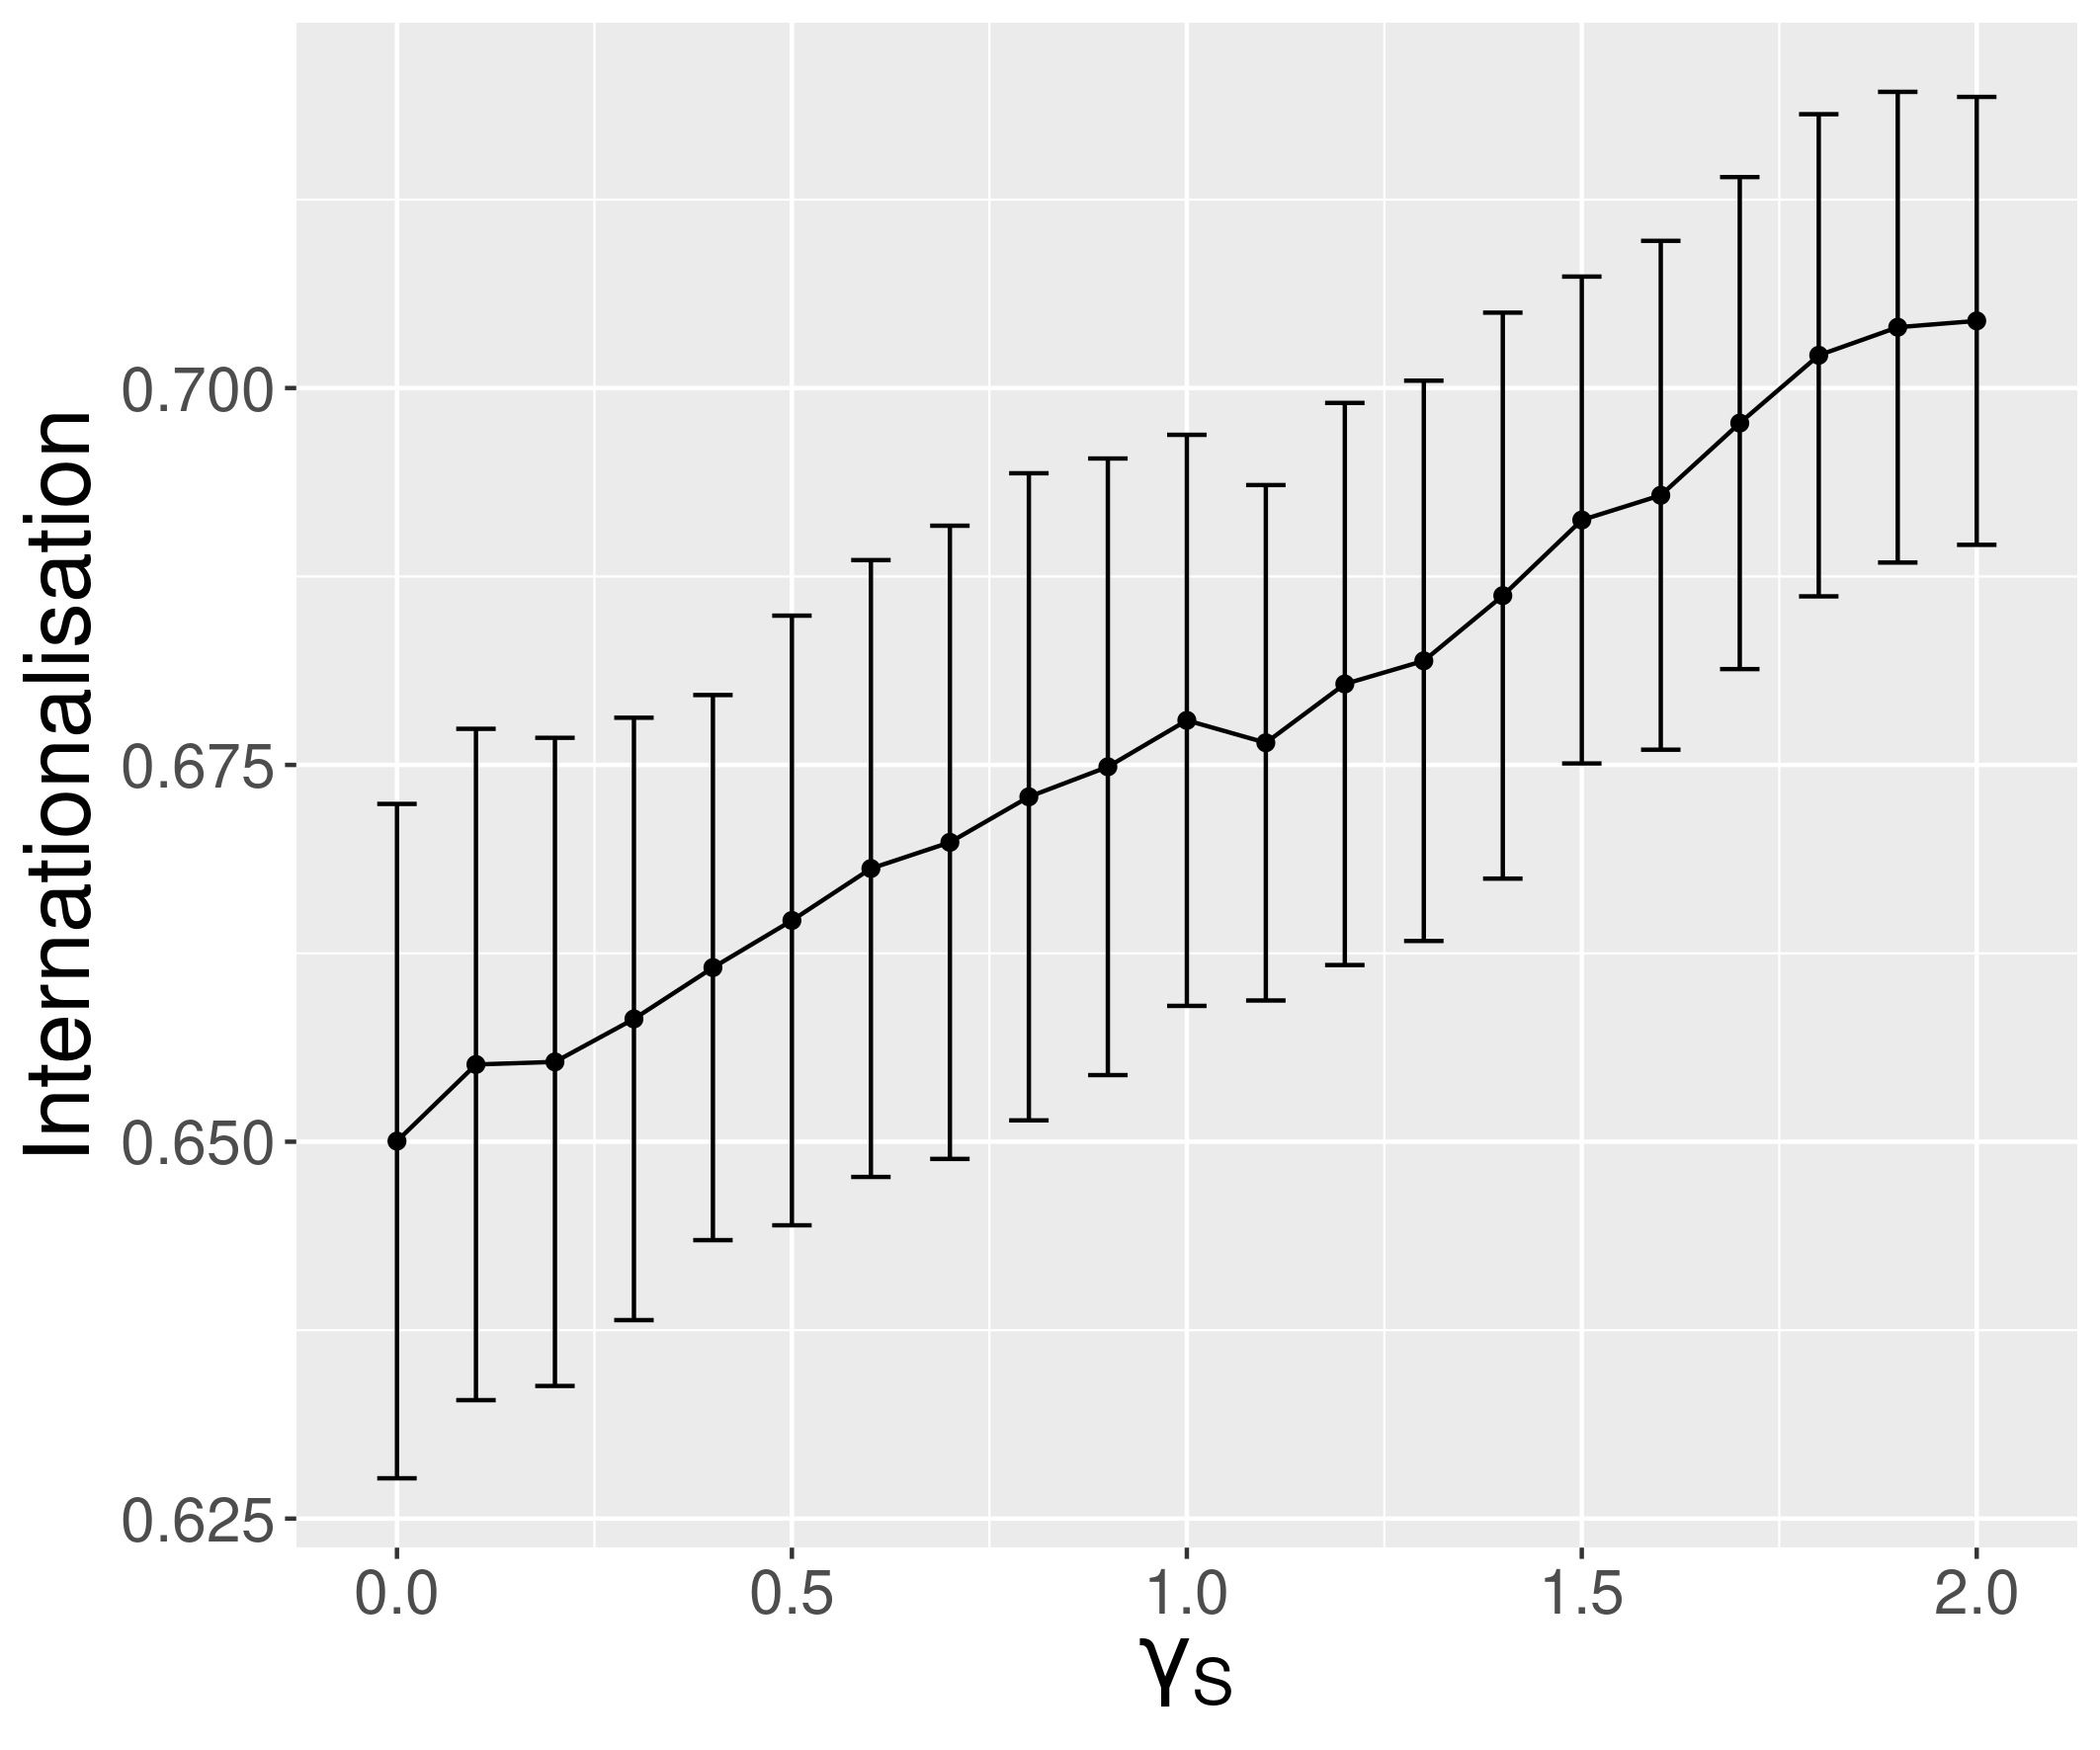
\includegraphics[width=0.48\textwidth]{figuresraw/internationalisation-gammaSectors_errorbars.png}
    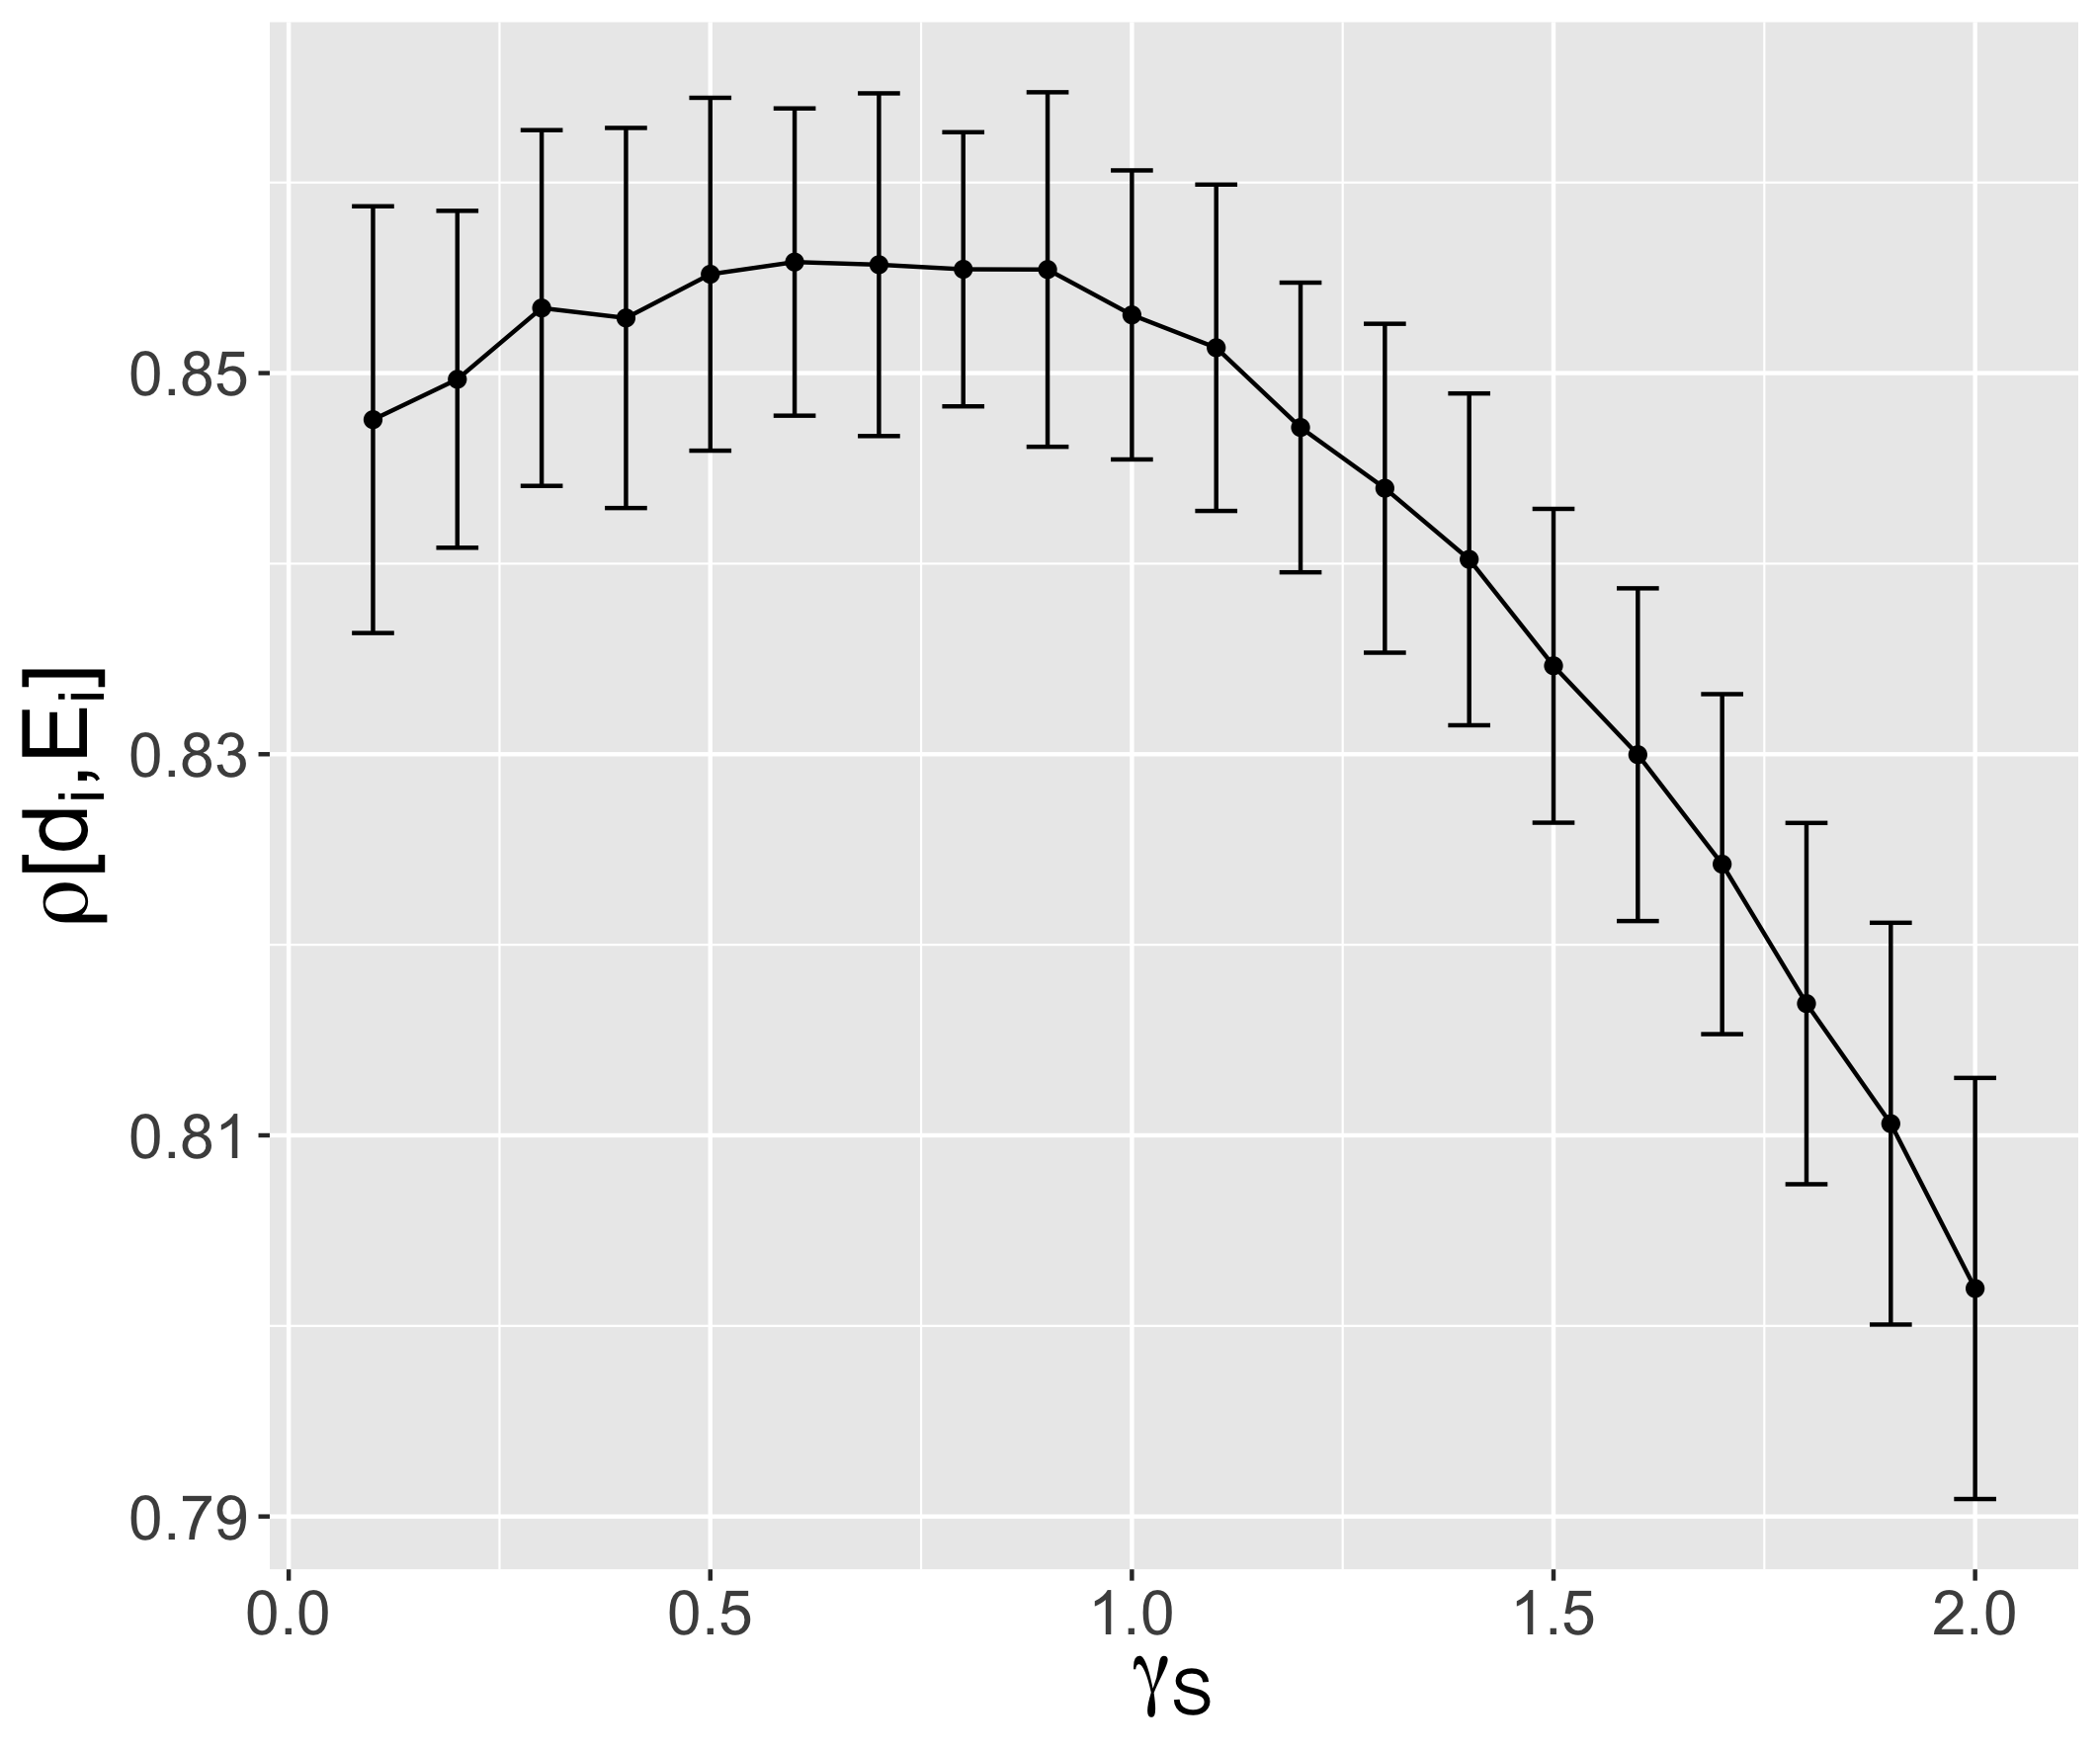
\includegraphics[width=0.48\textwidth]{figuresraw/rhoDegreeSize-gammaSectors_errorbars.png}
    
    \medskip
    \footnotesize
    
    \textit{(Left) Internationalization varies linearly with sector proximity $\gamma_S$; (Right) Correlation between degree and size exhibits a maximum, witnessing an intermediate regime where size is the most important}
    
    
}


\sframe{Grid exploration: internationalization}{

    \begin{center}
    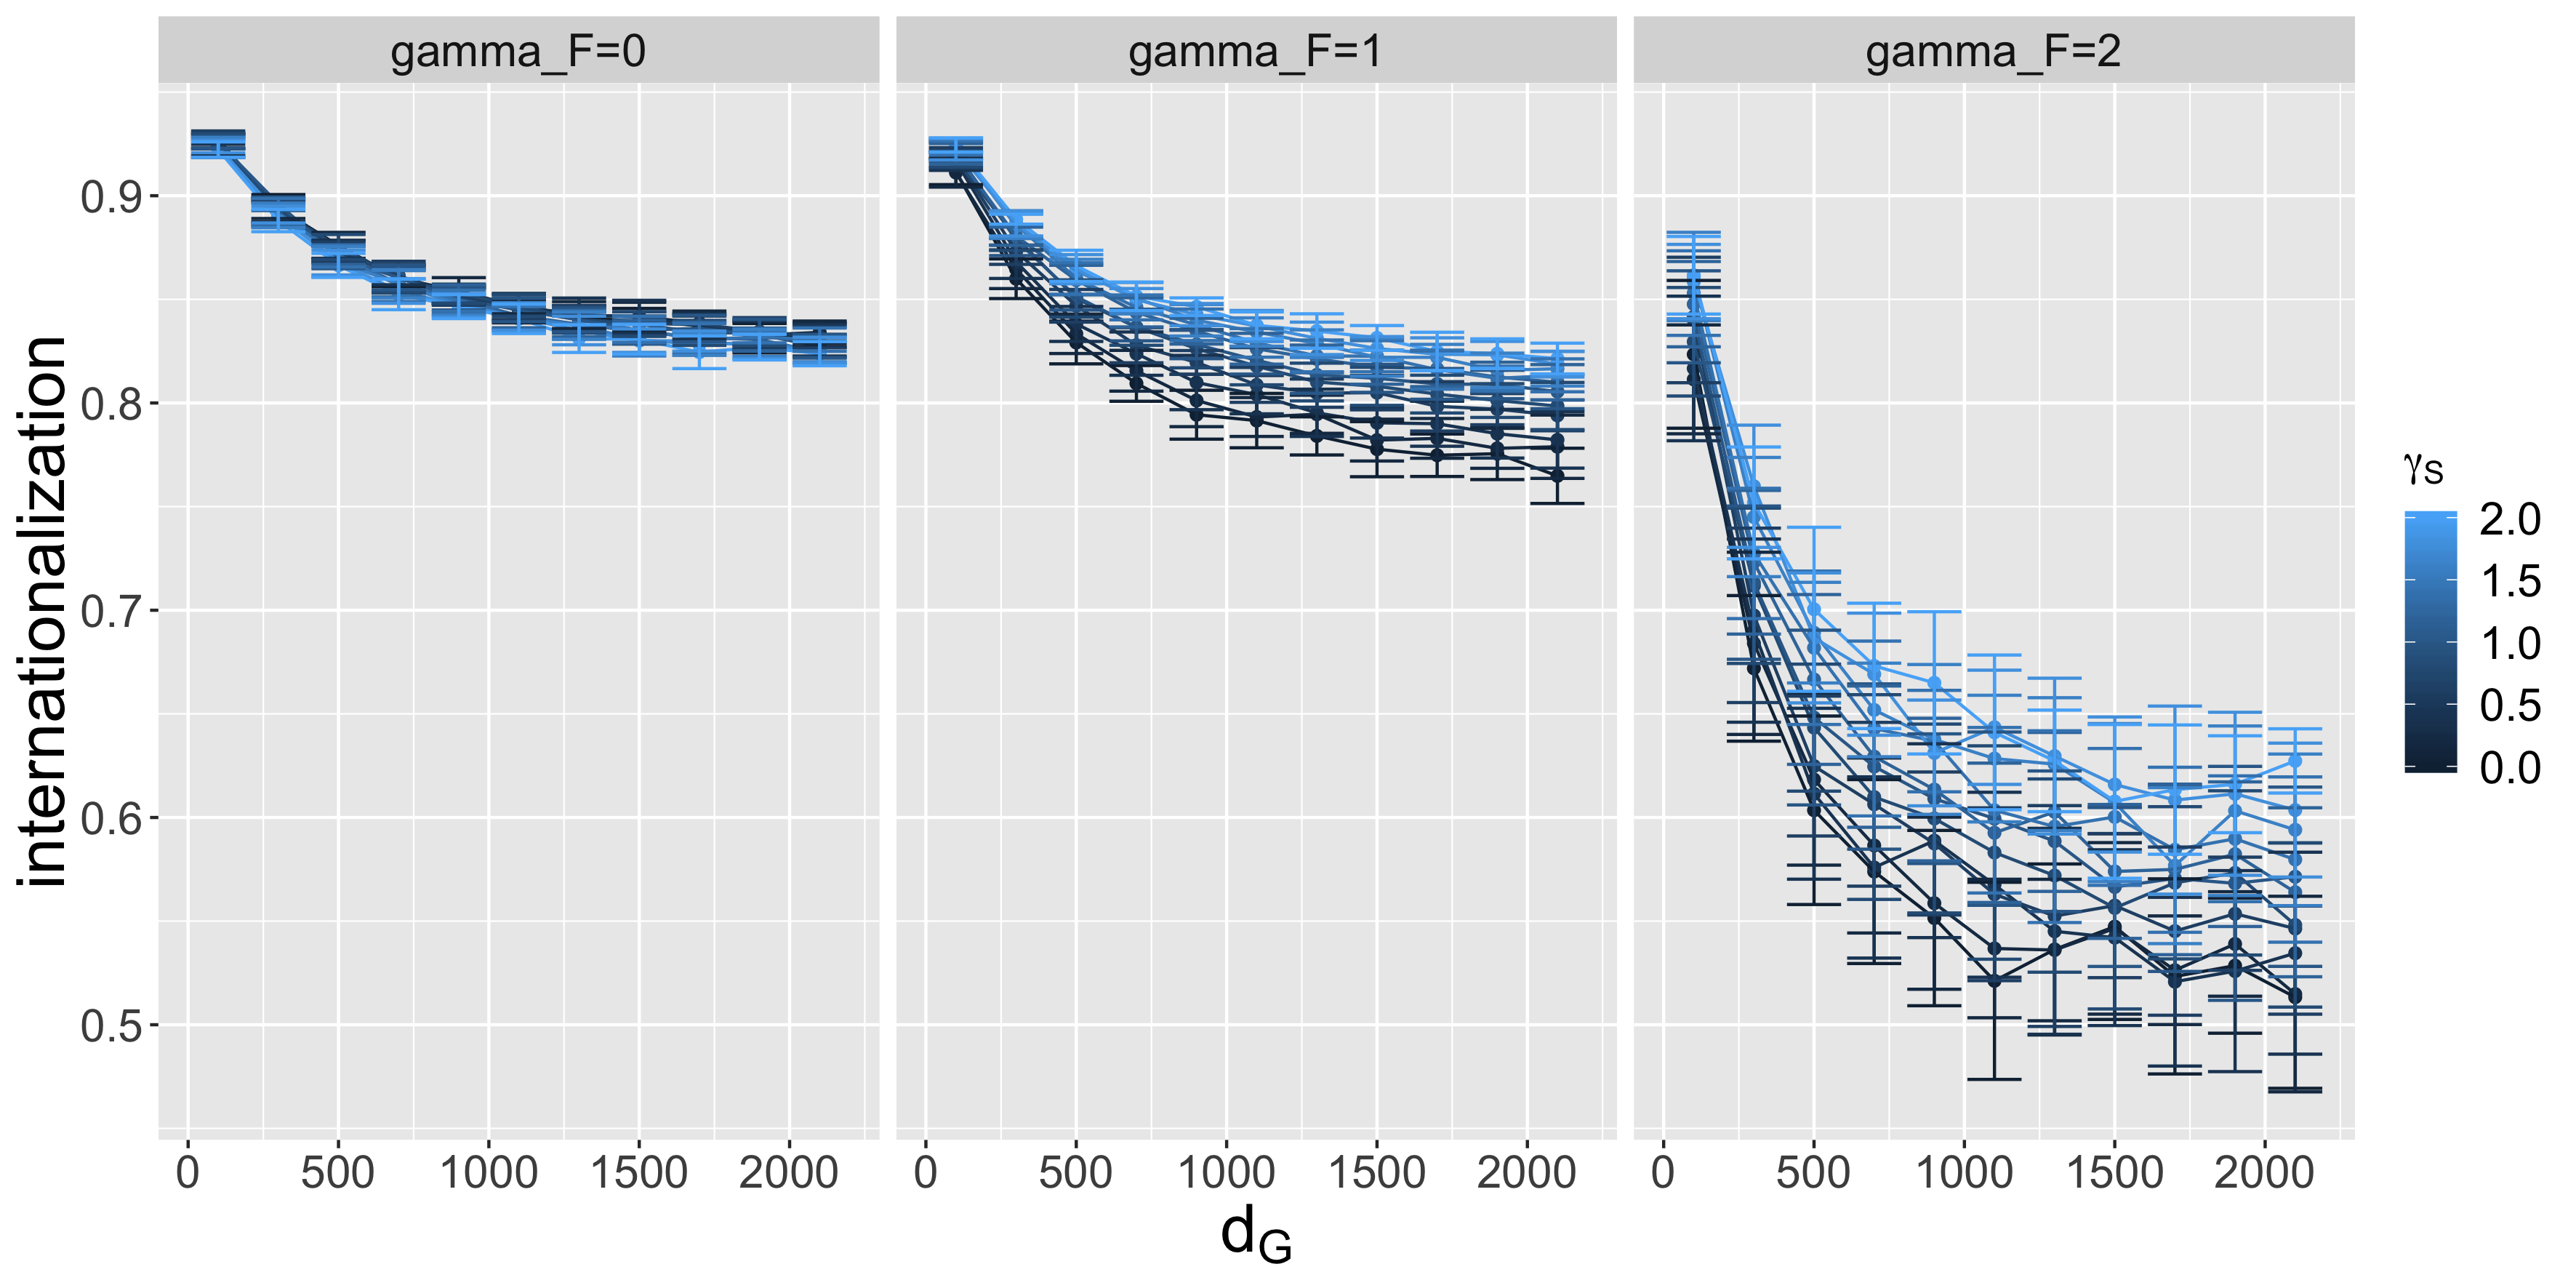
\includegraphics[width=\textwidth]{figuresraw/internationalization_countryGravityDecay200_gammaDestination0_facetwrapgammaOrigin_colorgammaSectors.png}
    \end{center}
    
    \medskip
    
    \footnotesize
    
    \textit{The transition as a function of interaction range depends on the influence of origin size $\gamma_F$; sector proximity $\gamma_S$ plays a role only for a large influence of the origin.}
    
}

% alors tu as explique pendant la presentqtion pour Mike, mais je n'ai pas compris pourquoi il a trois graphiques 0 1 2 et pourquoi le 3 est si different:?
% je pense qu'il faut reconmmer en un truc plus clair l'axe des ordonnees et les 0, 1, 2
% dG c'est quoi, c'est toujours le pqs de temps? donc la meme chose que le gravity decay?

\sframe{Grid exploration: community size}{

    \begin{center}
    	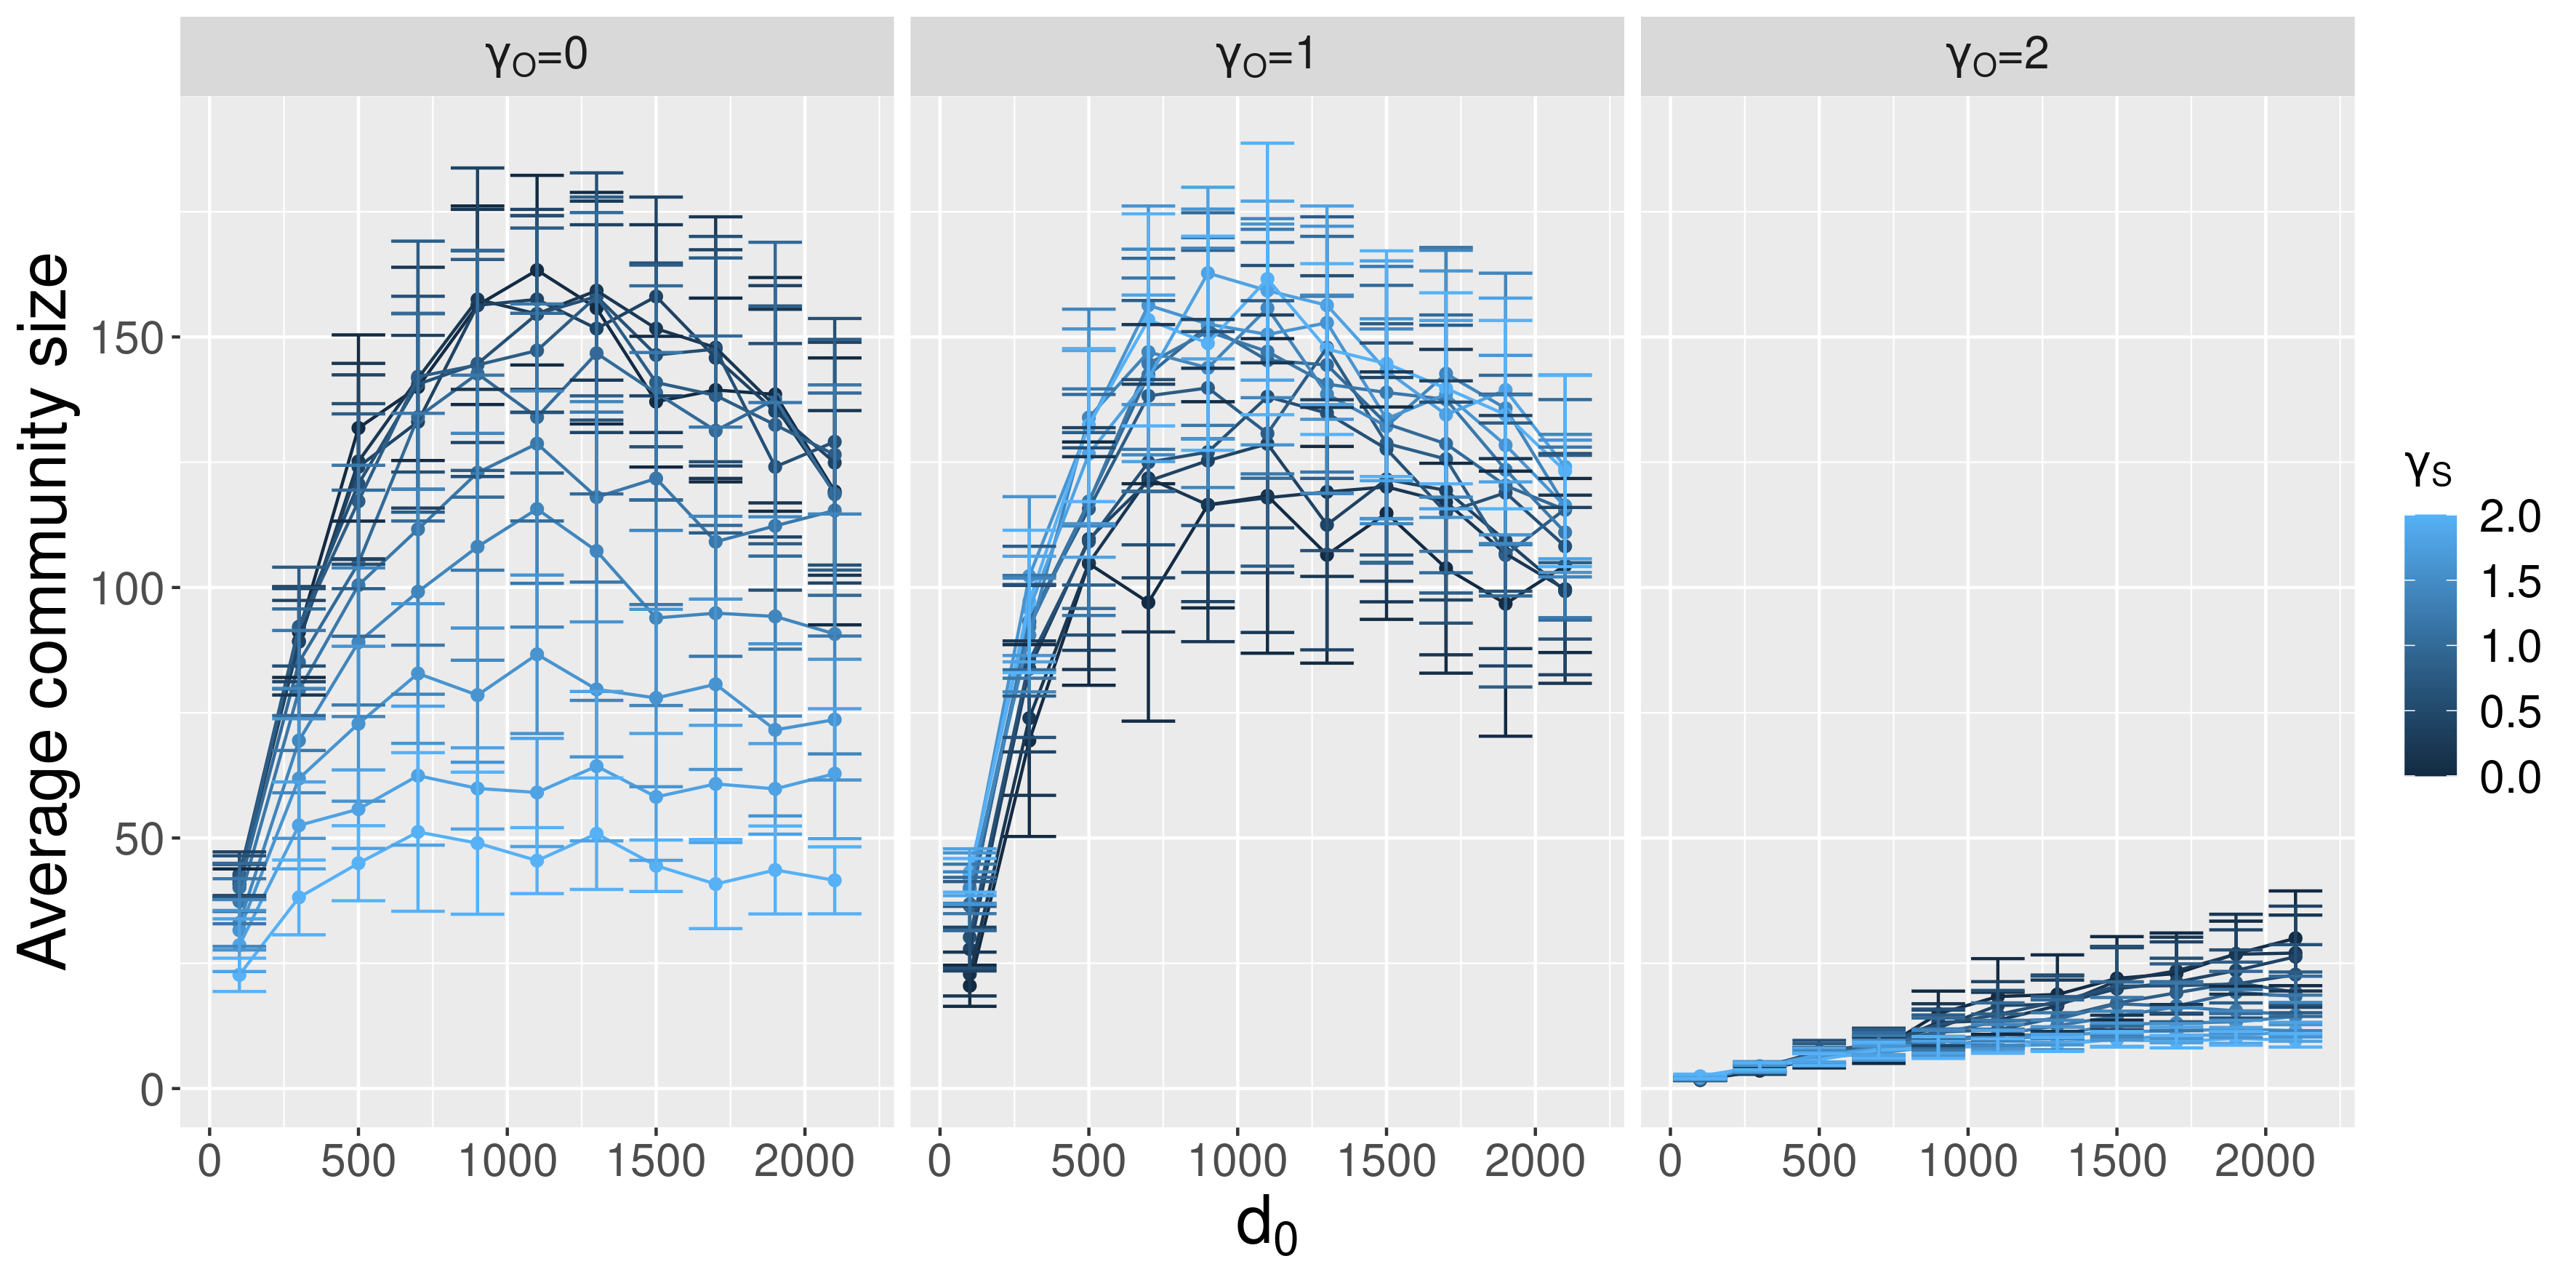
\includegraphics[height=0.6\textheight]{figuresraw/networkAvgCommunitySize_countryGravityDecay2100_gammaDestination0_facetwrapgammaOrigin_colorgammaSectors.png}
    	
    \end{center}
    
    \vspace{-0.5cm}
    
    \footnotesize

\begin{itemize}
	\item Maximal integration in term of community size is achieved at an intermediate value of $d_G$: emergence of a regional regime
	\item Maximal size depends on the role of sectors $\gamma_S$, in a decreasing way when origin size is deactivated, and increasing way when $\gamma_F=1$
	\item This regime disappear when origin size influence is too large
\end{itemize}
    
}

% alors ici il faut reconnomer l'axe des ordonnees ca peut etre community size? qui est defini comment d'ailleurs ici? C'est la ou tu as dit que le pic aussi rapide est interessant, donc en si peu de temps la taille du reseaux grossi c'est ca :'(? et du coup comment expliquer le 2 a droite? 


%\sframe{Grid exploration}{
%    \centering
%
%    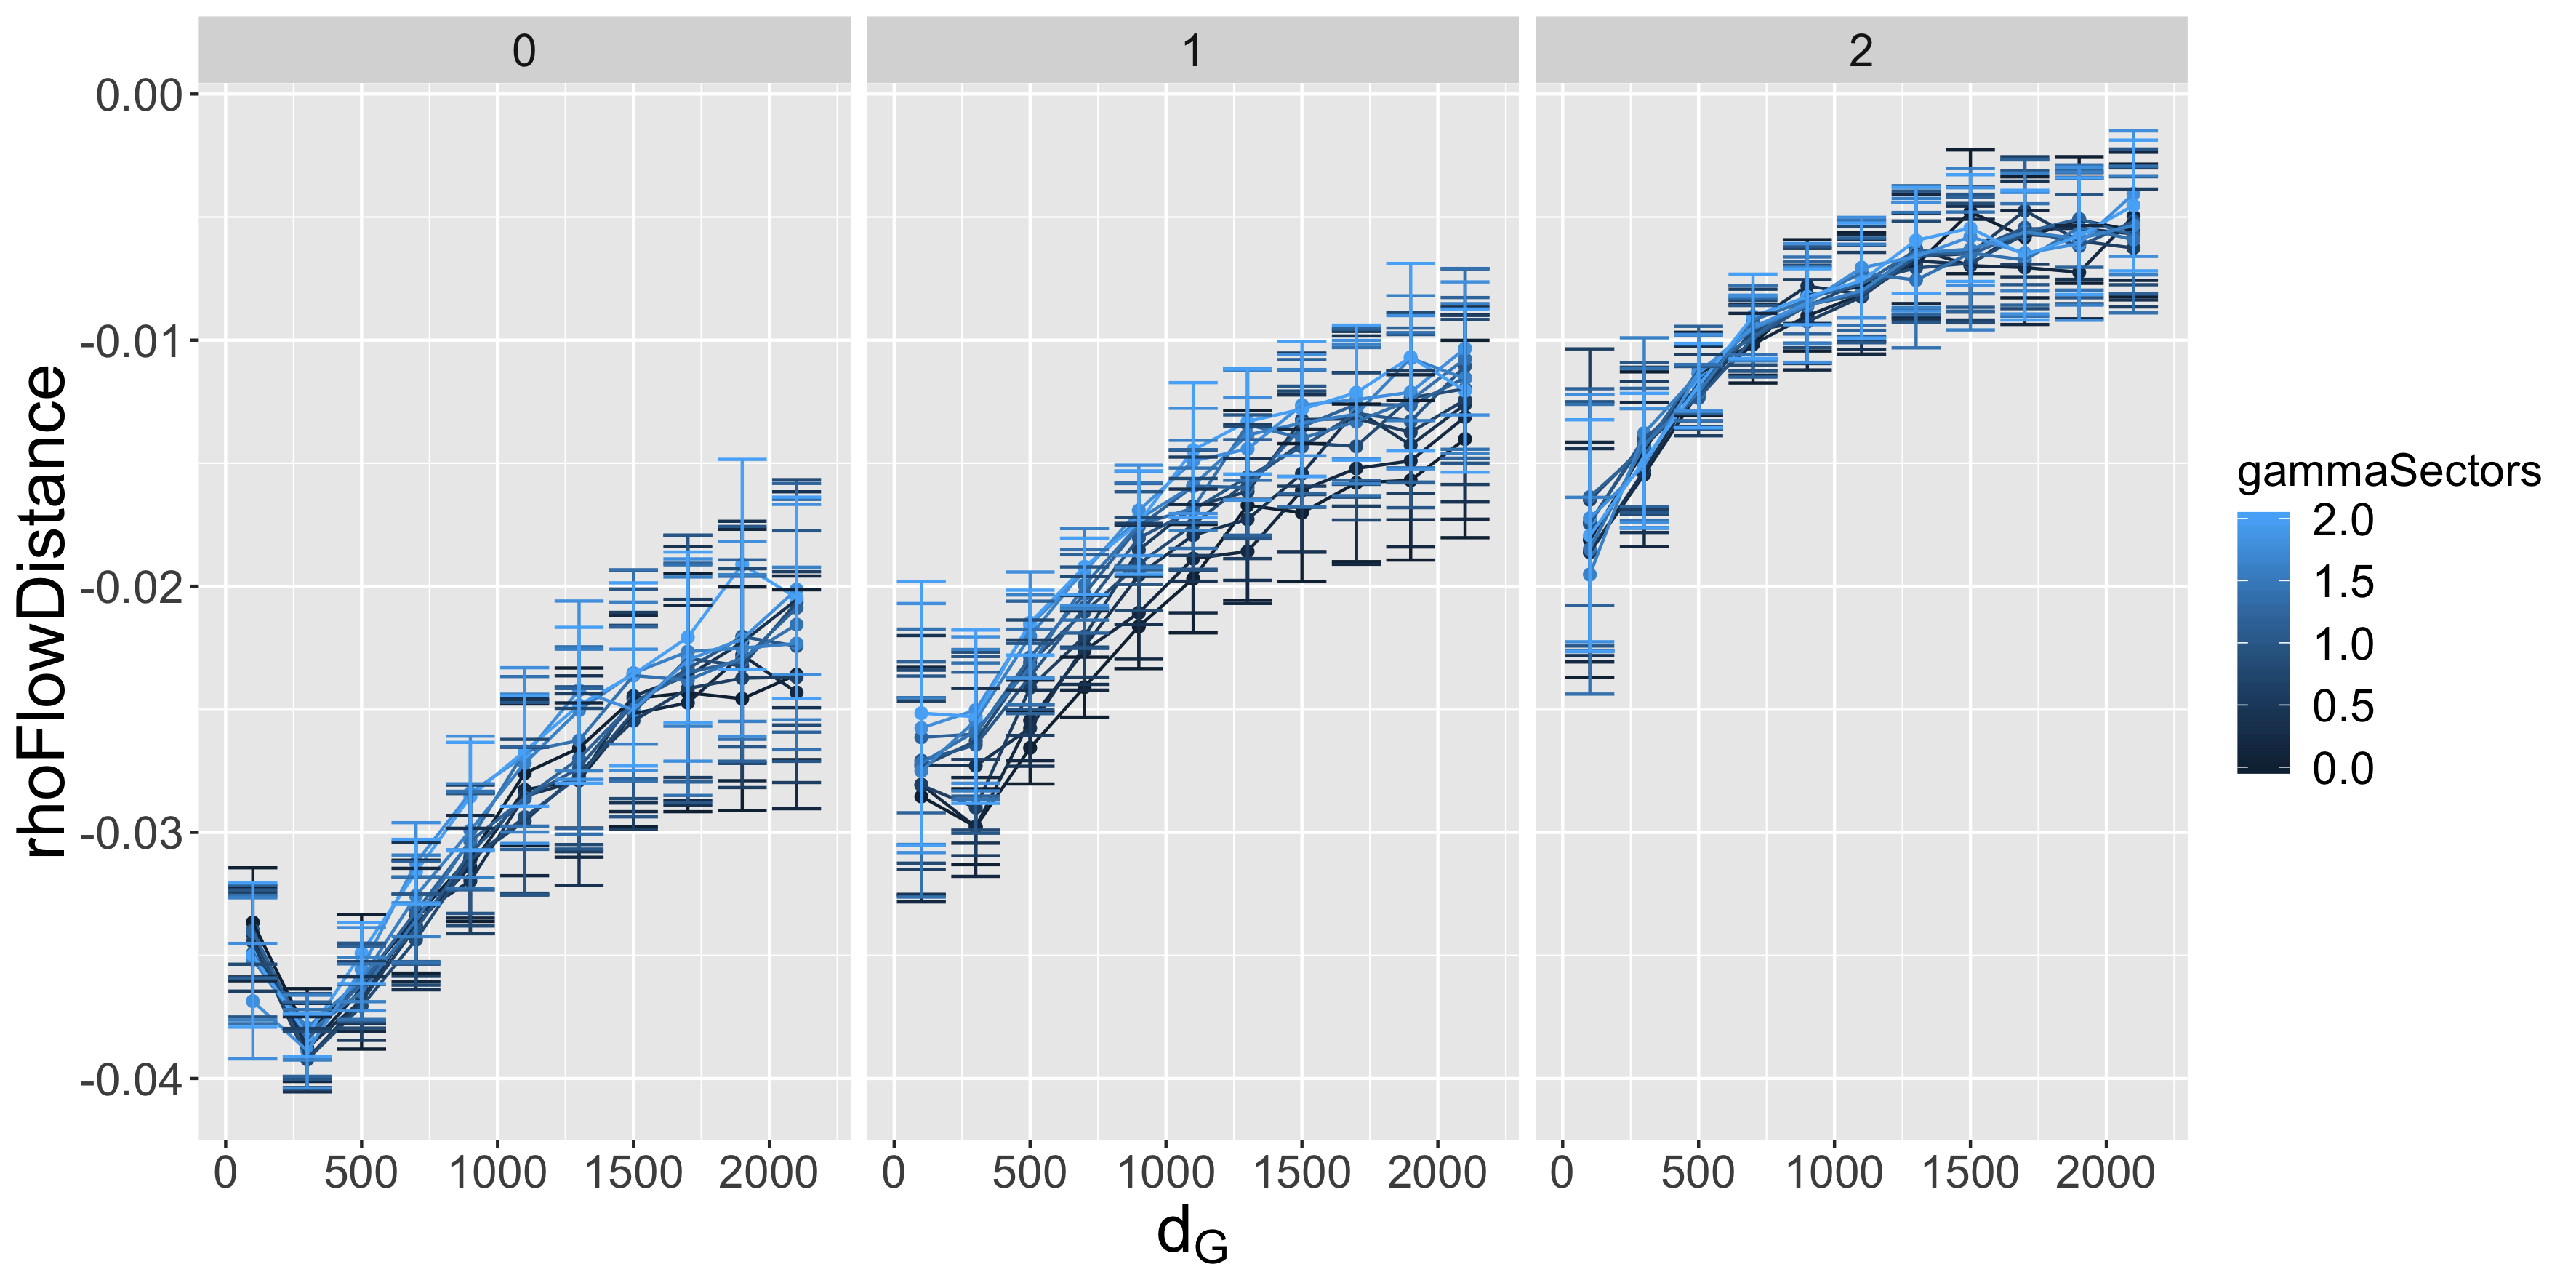
\includegraphics[width=\textwidth]{figures/rhoFlowDistance_countryGravityDecay2100_gammaDestination2_facetwrapgammaOrigin_colorgammaSectors.png}
%}

% idem la c'est pas facile a lire pour quelqu'un qui ne connait pas. c'est quoi rhoFlowDistance?
% le gamma sector c'est le parametre de la variable secteurs donc s? 
% en fait quand j'y pense pourquoi il yq u gradien du gamma et comment comprendre ces varations pour chqaue pqs de temps

% other experiments ? PSE on correlations ?




\section{Discussion}

% - future work etc (classical discussion)
% - on the role of model exploration and simulation to gain knowledge from the model

% further comparing with real data?



\sframe{Discussion}{

\justify
\footnotesize

\textbf{Practical application}

$\rightarrow$ effect of exogenous shocks in the socio-economic structure (``subsystem-xit'')

\medskip

\textbf{Developments}

$\rightarrow$ evolution of city sizes (co-evolution model)

$\rightarrow$ parametrization/calibration on real data

$\rightarrow$ role of path-dependency

$\rightarrow$ towards a model with firm agents? (multi-scale ABM)

\medskip

\textbf{On the role of model exploration}

$\rightarrow$ even with such a ``simple'' model (close to directly tractable stationary state), behavior is highly non-linear in many dimensions

$\rightarrow$ model exploration allows to overcome hidden parameters (deactivated mechanisms or default parameter values)

$\rightarrow$ exploration of intrinsic dynamics on synthetic data is a crucial step before an application on real data (disentangle effects of geography from model dynamics)






}


\sframe{Conclusion}{

$\rightarrow$ A generative model to understand processes of economic network emergence

\bigskip

$\rightarrow$ Crucial role of model exploration to validate and extract knowledge from such a simulation model


\bigskip
\bigskip


\textbf{Open repository for model and results at}

\texttt{https://github.com/JusteRaimbault/ABMCitiesFirms}

\bigskip

\textbf{Simulation data at} \texttt{https://doi.org/10.7910/DVN/UPX23S}

\bigskip

\textbf{Acknowledgments}: thanks to the \textit{European Grid Infrastructure} for access to the infrastructure.


}



%%%%%%%%%%%%%%%%%%%%%
\begin{frame}[allowframebreaks]
\frametitle{References}
\bibliographystyle{apalike}
\bibliography{biblio}
\end{frame}
%%%%%%%%%%%%%%%%%%%%%%%%%%%%







\end{document}

